\chapter{Improvements in the Analysis}

In the previous chapter, we had show examples where the heap liveness analysis applied to the synchronized control flow graph returned a highly-over approximated access graph. The reason for this being the inter-thread synchronization edges not being treated differently from intra-thread edges. There is also a need to ensure that the final data flow value obtained can actually be a result of valid program execution. \\

In order to achieve this we need to analyze critical sections in all the threads. An intra-thread analysis will be required to be performed. We need to figure out the whether there exists a loop outside the critical section. If there is no such loop then we can say that the critical section will be executed once. Otherwise, The critical section can be executed zero or more times. Note that this information in thread independent. Once we have the thread dependent information , we can add inter-thread edges. The edges will only be triggered based on the condition that checks if the critical section can be executed. The condition would involve comparing counters of the number of times a critical section is executed. \\

One way to achieve this is to label the edges with the number of times the transition is possible. Considering the examples in the last chapter figure 5.1, 5.2 and 5.3, we can suggest the following access graphs at the statement main(). See figure 6.1. \\


\begin{figure}
	\centering
	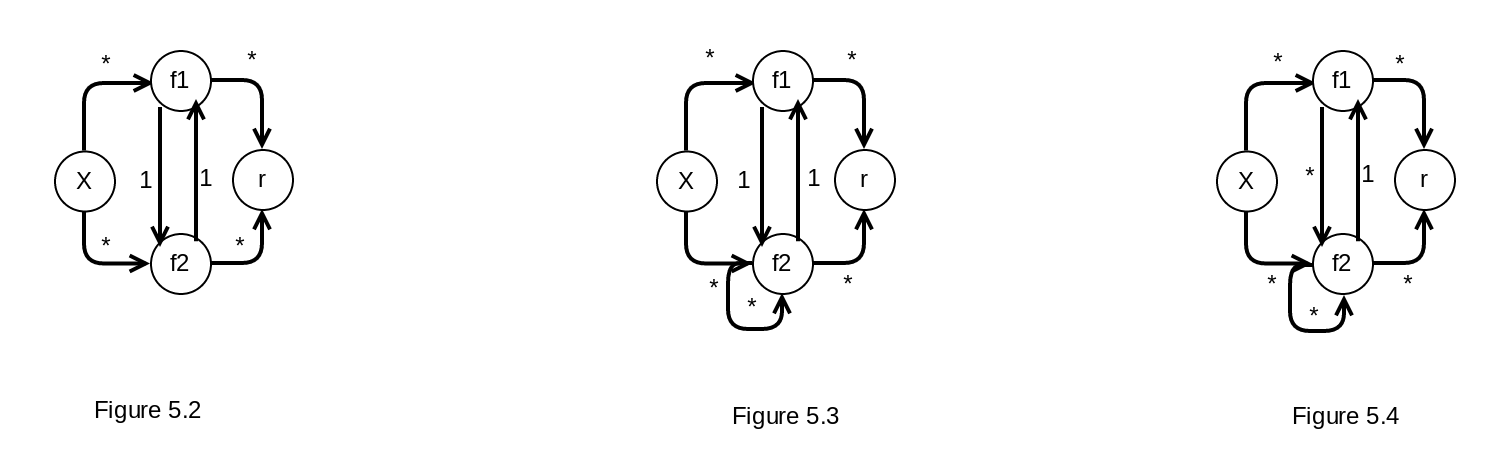
\includegraphics[width=0.8\textwidth]{Figures/access_graph_rep.png}
	\caption{Desired Access graphs for fig 5.2,5.3 and 5.4}
	\label{fig:ch5example}
\end{figure}
 
In examples 5.2,5,3 and 5.4 , we had observed that access graph at the statement main() was the same. We now display the desired representation of access graph. For example 5.2, we have observed that the critical section can only be executed once for both the threads. So we need to mark the edge with either 1 or *, where 1 denotes that the transition can only be performed once and * is a doesn't care condition. \\

For 5.3, we had a loop inside critical section of thread 2. However the critical section could only be executed once. There will be a self loop around $f_2$ in the access graph. The edges from $f_1$ and $f_2$ are representative of a thread change. Since there are no loops across/outside the critical section, we can conclude that both these will execute once and mark the two edges 1. \\

For example 5.4, there is a thread 2 has a loop across the lock and unlock section. Thus now the edge representing transition from $C_1$ to $C_2$ can be executed any number of times. The desired access graph for 5.4, should be the similar to 5.3 except for the edge from $f_1$ to $f_2$ being labeled as * instead of 1. \\

We may need to modify the analysis in order to obtain the desired access graph for all the examples. One way may be to change the way we merge and summarize access graphs different threads. Another way could be   

\section{Concurrent Heap Access examples}

Let us try to understand the how heap memory is actually accessed by threaded programs using shared memory. This will be better understood by taking up the example of a concurrent data structure say tree. Each node of the tree has \emph{left} and \emph{right} fields pointing to children and a \emph{data} field.   